\section{Knowledge Representation}
\label{sect:knowledge}
%
\begin{algorithm}[h!]
\begin{tabbing}
\hspace*{.5cm}\=\hspace*{.5cm}\= \hspace*{.5cm}\= \kill
(:action place-part\\
\>	:parameters(\\
\>\>	?robot - Robot\\
\>\>	?stockkeepingunit - StockKeepingUnit\\
\>\>	?endeffector - EndEffector\\
\>\>	?kit - Kit)\\
\>	:precondition(and\\
\>\>	(endEffector-has-heldObject ?endeffector ?stockkeepingunit)\\
\>\>	(robot-has-endEffector ?robot ?endeffector)\\
\>\>	(equal-to (slot-found-flag) 1)\\
\>\>	(kit-has-slot ?kit))\\
\>	:effect(and\\
\>\>	(not(endEffector-has-heldObject ?endeffector))\\
\>\>	(set-value (slot-found-flag) 0)))\\
(:action look-for-slot\\
\>	:parameters(\\
\>\>	?robot - Robot\\
\>\>	?stockkeepingunit - StockKeepingUnit\\
\>\>	?kit - Kit)\\
\>	:precondition(and\\
\>\>	(equal-to (slot-found-flag) 1))\\
\>	:effect(and\\
\>\>	(set-value (slot-found-flag) 0)))\\
\end{tabbing}
\caption{Actions}
\label{fig:Actions}
\end{algorithm}
%
Two typical PDDL commands of {\it place-part} and {\it look-for-slot} 
are shown in Figure \ref{fig:Actions}. The {\it place-part} command
is used to put the currently held object into the ``slot'' of the kit
under construction that was found with the {\it look-for-slot} command.
If we assume that the action
{\it place-part} is being executed, then in line 4 of the {\sc BuildKit} algorithm
each of the predicates from the precondition section of the action 
will be verified. As previously mentioned, the evaluation of these predicates
could be hard-coded into the system. However, is there a more flexible way
that this could be accomplished?

\subsection{Predicate Representation}
If one examines each of the predicates that must be evaluated, it may be
noted that the predicates could be composed of a combination of simpler 
expressions. For example, the predicate expression:
\begin{gather} 
\class{endEffector-has-heldObject}(\textit{endeffector}, 
\textit{stockkeepingunit}),
\label{equation:endEffector-has-heldObject}
\end{gather}
is designed to verify that the robot's end-effector is holding the correct lass of part. It may be decomposed into the compound expression: 
\begin{gather}
\textbf{matchSKU}(\textbf{In-Contact-With}(\textit{endeffector}), stockkeepingunit)
\label{equation:matchSKU}
\end{gather}
In this case, \textit{endeffector} is the instance of the class end effector
that is expected to be attached to the robot
and 
\textit{stockkeepingunit} is the instance of the stock keeping unit
that belongs to the part that is expected to be held by the robot.
The expression \textbf{In-Contact-With} will determine what class of object is being held by the effector, while the expression \textbf{matchSKU} will determine if this represents the expected class.
 
The expressions \textbf{In-Contact-With} and \textbf{matchSKU}
are known as Intermediate State Relations (ISR) because the relate
complex elements of the system's state to easily measurable or
observable phenomenon. When called with a single parameter,
the measurable ISR of 
\textbf{In-Contact-With}(\textit{endeffector}) will return
a list of objects that are in contact with the end effector. 
This list will be passed as parameters to the observable
ISR of \textbf{matchSKU}. Since this relation is
expecting exactly two parameters, an end effector touching
zero or more than one object will result in an error. If a
single object is being held, it will be passed to \textbf{matchSKU} where
a simple observation may be made to see if the object's SKU
matches the one provided in the second parameter.

\subsubsection{RCC-8 Relation}
All of the measurable intermediate state relations may be further
decomposed into expressions that may be easily computed from
knowledge of the six degree-of-freedom pose of the objects. 
These base expressions are know
as Region Connected Calculus (RCC-8) relations and were originally
developed by Wolter and Zakharyaschev \cite{Wolter2000} 
as an approach for representing the relationship between two regions in 
Euclidean or topological space. 
RCC-8 consists of eight possible relations (hence RCC-8) that include
measurable region-to-region relationships such as
Tangential Proper Part (TPP) and Externally Connected (EC). 

In order to represent these relations in all three dimensions for 
industrial domains, RCC-8 has been extended to a three-dimensional space 
by applying it along all three planes (x-y, x-z, y-z) and by including 
cardinal direction relations ``+'' and ``-''. In our example of
Equation \ref{equation:matchSKU}, 
\textbf{In-Contact-With}(\textit{endeffector}) may be expressed
in RCC-8 relations as:
\begin{gather}
\textbf{In-Contact-With}(\textit{obj1}, \textit{obj2}) \rightarrow   \notag\\
\texttt{x-EC}(\textit{obj1}, \textit{obj2}) \vee \texttt{y-EC}(\textit{obj1}, \textit{obj2}) \vee \texttt{z-EC}(\textit{obj1},\textit{obj2}) \notag
\end{gather} 
Where \textit{EC} stands for Externally Connected, obj1 is the end effector, and obj2 is 
cycled through all of the detected objects in the work cell. 
\subsection{Observable Relations}
Work is still being performed to relate all of the simple observations to observable relations. In the case of the \textbf{matchSKU} observation, a \textit{model-match} or \textit{view-sku} operation could be performed. More on this topic is presented in Section \ref{sect:future}.
\subsection{Action Execution}
Once the precondition predicates have been validated, line 8 of the \textsc{BuildKit}
algorithm in Figure \ref{fig:buildkit} shows that the action should be executed. Once
again it is possible to decompose the complex actions into a much simpler form. 
In this case, two separate basis sets exist with one designed for the decomposition 
of Robot Actions and the other for the decomposition of Vision Actions.
%
\begin{figure}[htb!]
\begin{center}
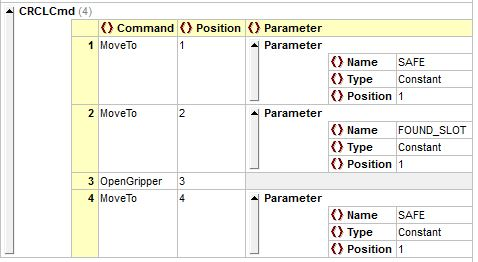
\includegraphics[width=8.5cm]{images/PlacePartCRCL.jpg}
\caption{The \textit{place-part} action may be decomposed into a sequence of
four CRCL commands.} 
\label{fig:PlacePartCRCL}
\end{center}
\end{figure}
%
\subsubsection{Canonical Robot Command Language}
The National Institute of Standards and Technology (NIST) has developed a
robot language known
as the Canonical Robotic Command Language (CRCL) that is designed to provide
a basis set of operations for robotic arms with industrial use 
cases \cite{Balakirsky2012-1}. This language contains 22 command elements that
may be sequenced to perform any of the PDDL Robot Actions that have been defined
for this domain. Continuing our example from above, 
Figure \ref{fig:PlacePartCRCL} displays the decomposition of the \textit{place-part} action.
As may be seen in the figure, the command decomposes into several movements and a gripper
command. The movements to a ``safe" location are not strictly necessary, but are
included to assure that the arm's motion begins and ends from a known safe position.
This position is a predefined constant in the system.
\textit{FOUND\_SLOT} is another system constant that represents a position buffer in 
the system. This buffer has previously been filled with the location of the actual
slot that is the destination of the part with the PDDL action 
\textit{look-for-slot}. 

Once the command execution is complete, the predicates that make up the effects
are examined in the same manner as the previously examined precondition predicates.
If any of the effects are deemed to have not occurred, then an error will be
generated.
\subsection{Instance Representation}
\label{sect:instance}
As discussed in the previous section, all of the PDDL predicates and actions may be
decomposed into a small set of primitives that includes
Robot Actions, Vision Actions, RCC-8 relations, and Observables. 
If this set of primitives is
programmed into the robot cell, then the set of behaviors that the cell is capable of
may be altered through the creation of new PDDL actions and predicates rather than
reprogramming the cell. In addition, these PDDL actions and predicates are independent
of the actual cell's implementation and product vendors. As long as the cell supports the
full set of primitives, it is capable of carrying out the operations without programming.

In order to translate PDDL predicates and actions into robot cell commands, 
the executor needs to have an
understanding of how the predicates and actions are composed. Since this information is
designed to not be hard-coded on the robot, it must be accessible to the running system.
In addition, since the actions and predicates are designed to be expanded upon as
new activities are added to the robot's vocabulary, the information needs to be
accessible in a human friendly form.
%
\begin{figure}[htb!]
\begin{center}
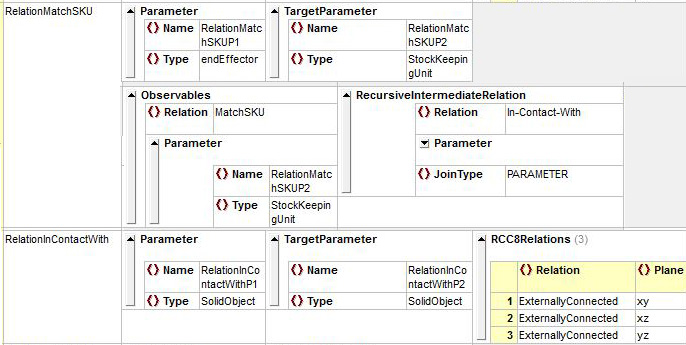
\includegraphics[width=12cm]{images/MatchSKU_ISR.jpg}
\caption{Intermediate State Relation RelationMatchSKU. This is the
implementation of Equation \ref{equation:matchSKU}.}
\label{fig:ISR}
\end{center}
\end{figure}
%
To meet all of these demands, this information is encoded in the Instance Ontology and is automatically entered into the Execution Model's MySQL database. 

The primitives themselves are implemented as simpleTypes in the schema.
In this case, the XML simpleType specifies an enumerated list of terms
that are within the robot and vision system's vocabulary. All of the
ISRs, predicates, and actions are composed of these elements, and these
elements are the only part of the system that is hard-coded onto the
robot.
\subsubsection{Intermediate State Relation}
The structure of the RelationMatchSKU ISR required by Equation \ref{equation:matchSKU} is shown in the XML
representation
depicted in Figure \ref{fig:ISR}. 
Recall from Equation \ref{equation:matchSKU} that this ISR is 
a recursive combination of the Robot ISR \textbf{In-Contact-With} and
the Vision ISR \textbf{MatchSKU}. This is shown in the XML in that
the \textit{RecursiveIntermediateRelation} is instantiated as
\textbf{In-Contact-With} with a single parameter of the end effector
and the \textit{JoinType} of \textit{PARAMETER}. This will cause a determination
of every object that is in contact with the effector. The 
determination of which objects are in contact with the effector
is made through the application of RCC-8 relations as shown in
the bottom part of Figure \ref{fig:ISR}. In this case, three
externally connected relations must be evaluated for each
object.The list of objects in contact
will get passed back as parameters to the \textit{MatchSKU} Vision ISR.
If zero or greater than one objects are passed to \textit{MatchSKU},
an error will be generated. If and only if one object is passed as
a parameter, that object's SKU will be compared against the target
SKU. Thus, from a combination of primitives we are able to determine
if the object being held by the end effector matches the SKU of the
expected object class. This in turn will deliver the truth value
of the predicate \textit{endEffector-has-heldObject()} depicted
in Equation \ref{equation:endEffector-has-heldObject}.  
\subsubsection{Actions}
\textit{CRCLActionTypes} and \textit{VisionActionTypes} are included
in the xml schema and are extensions of the \textit{ActionType} depicted
in Figure \ref{fig:ActionType}. These actions add the list of CRCL commands or observations that are required for the execution of the action. A sample of the CRCL commands for the \textit{place-part} action
are shown in Figure \ref{fig:PlacePartCRCL}. The encoding of all of the
actions is performed in the instance ontology.
